\documentclass[10pt,a4paper]{article}
\usepackage[latin1]{inputenc}
\usepackage{amsmath}
\usepackage{amsfonts}
\usepackage{amssymb}
\usepackage{graphicx}
\author{Raul Persa, Lukas Vogel}
\title{Feature Overview}
\begin{document}
	\maketitle

\textbf{Note:} at all times, the displayed election can be changed via the toggle on the top right or by changing the electionID parameter in the URL. 


\section*{Analysis}
\subsection*{Overview}
	
	\includegraphics*[scale=.2]{overview.png}
	
	\textbf{reachable via \texttt{/wahlanalyse/<electionID>}} or directly via the \"Ubersicht button on the navigation header. \\
	
	It shows the composition by seats of the chosen election as half donut chart and as table. A bar chart comparing the results with the election before (if available) is also shown.
	
\subsection*{Abgeordnete}
	\includegraphics*[scale=.2]{abgeordnete.png}
	
	\textbf{reachable via \texttt{/wahlanalyse/<electionID>/abgeordnete}} or directly via the Abgordnete button on the navigation header.\\
	
	All representatives that won a mandate are listed together with their Bundesland and party (if applicable). If they won a direct mandate, their Wahlkreis is also displayed as hyperlink leading to an overview of the Wahlkreis.


\subsection*{Wahlkreise}
		\includegraphics*[scale=.2]{wahlkreise.png}
		
		\textbf{reachable via  \texttt{/wahlanalyse/<electionID>/wk}} or directly via the Wahlkreise button on the navigation header.\\
		
		All constituencies are listed here together with the parties that won the first/second vote. Clicking on a table row leads to an overview of the constituency.


\subsection*{Wahlkreis�bersicht}
		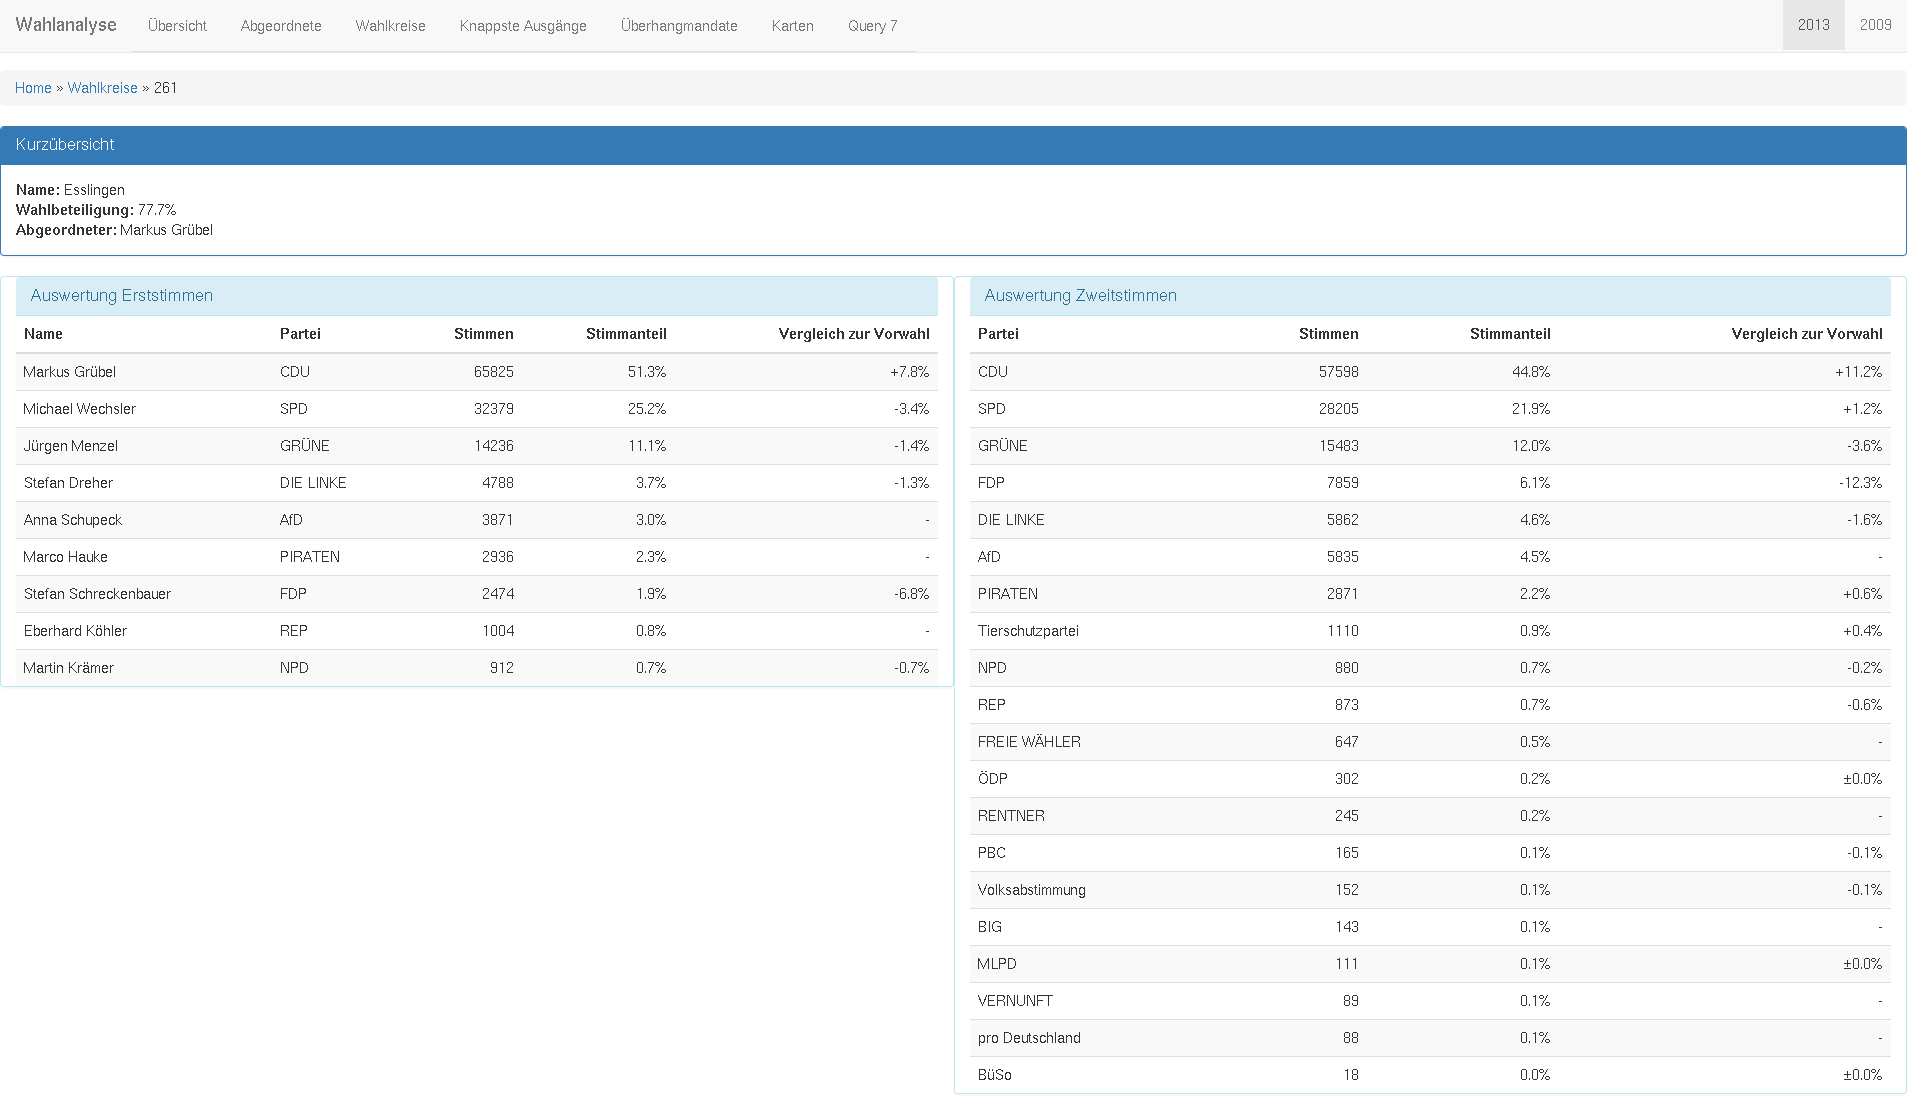
\includegraphics[scale=.2]{wahlkreis_overview.png}
		\textbf{reachable via  \texttt{/wahlanalyse/<electionID>/wk/<wahlkreisID>}} or by clicking on an element in the Wahlkreise list.\\
		
		The following information is shown:
		
		\begin{description}
			\item[Kurz�bersicht] Showing the most important information: Name of the constituency, percent of voters participating and the winning candidate.
			\item[Auswertung Erststimmen] The electable candidates, their party (if any), votes, percentage of votes and comparison to the previous election (by party).
			\item[Auswertung Zweitstimmen] The parties with a Landesliste in the Bundesland of the constituency, votes , percentage of votes and comparison to the previous election (if one exists).
		\end{description}
		
\subsection*{Query 7}		
		\textbf{reachable via  \texttt{/wahlanalyse/<electionID>/q7/<wahlkreisID>}} or directly via the Query7 button on the navigation header.\\
		
		Shows the same information as the Wahlkreis�bersicht but on unaggregated data. To see the result for other constituencies, change the wahlkreisID in the URL.
\subsection*{Knappste Sieger}
		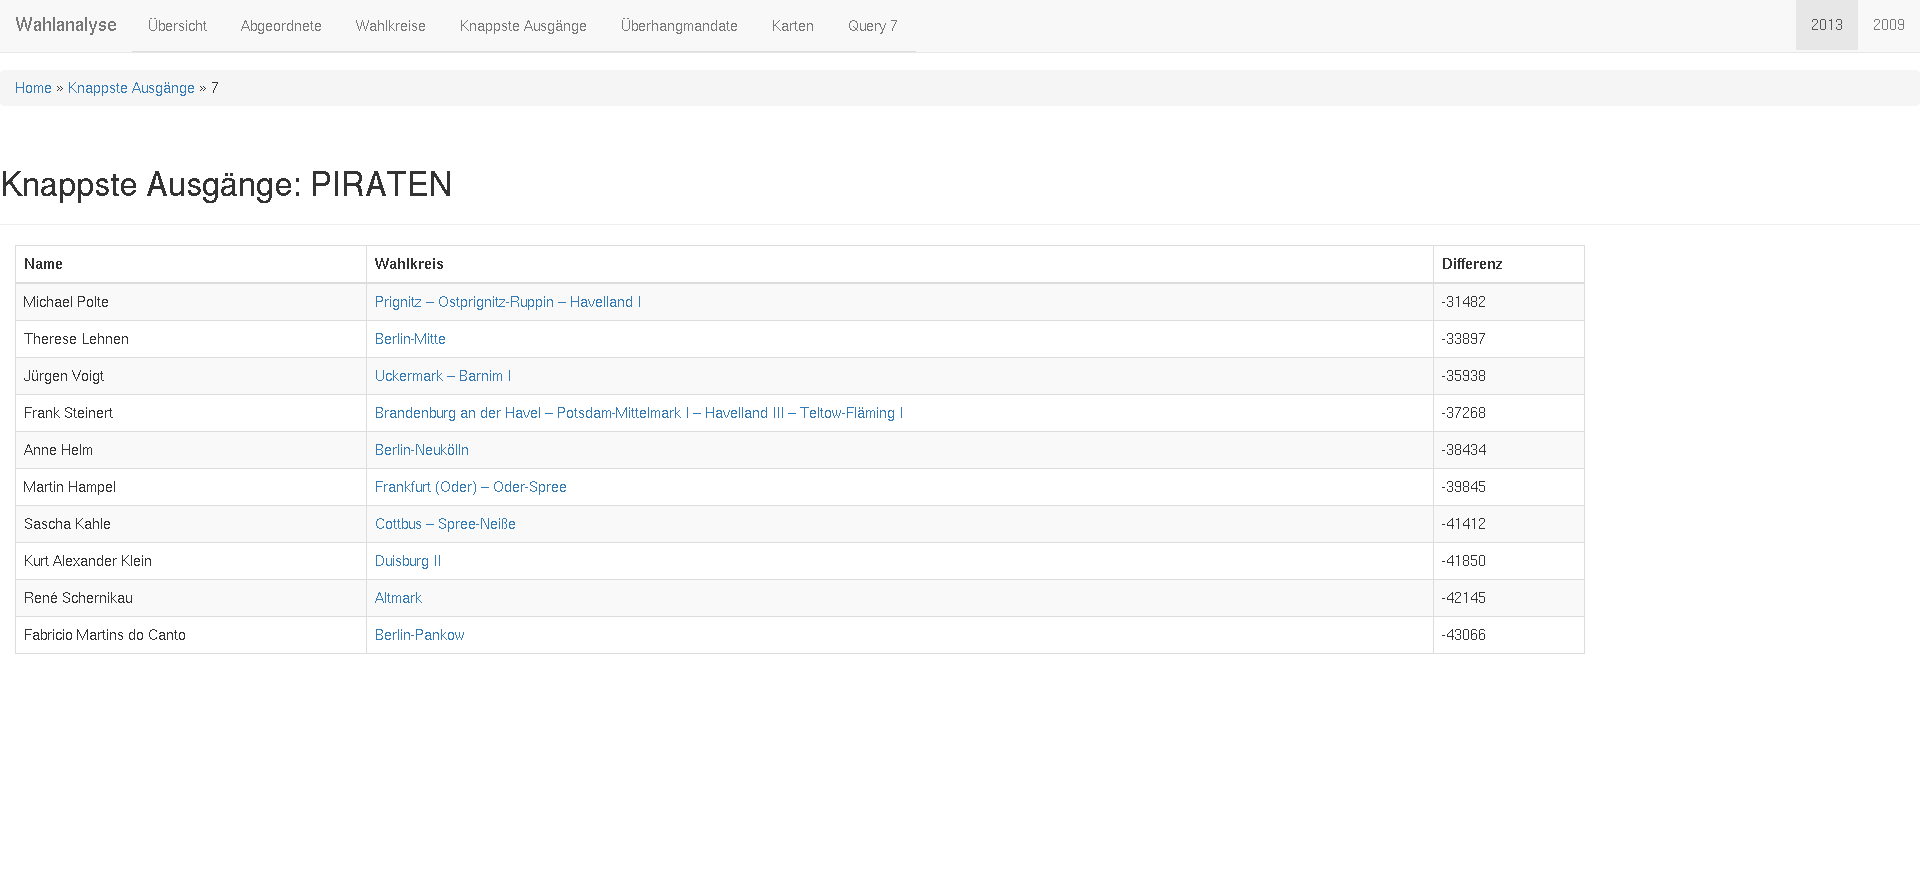
\includegraphics[scale=.2]{knappste_sieger.png}
		
		\textbf{reachable via \texttt{/wahlanalyse/<electionID>/ks/<partyID>}} or directly via the Knappste Ausg\"ange button on the navigation header. \\
		
		Showing the closest winners for each party. If no candidate of the party has won a constituency, the 10 closest losers are shown instead.
		If navigating through the menu or leaving out the partyID, a party has to be chosen first.
		
		
		
\subsection*{�berhangmandate}
		\includegraphics*[scale=.2]{ueberhangmandate.png}
		\textbf{reachable via \texttt{/wahlanalyse/<electionID>/ueh}} or directly via the \"Uberhangmandate button on the navigation header. \\
		
		All overhang mandates grouped by bundesland and party are shown.
		
\subsection*{Karten}
		\includegraphics*[scale=.2]{karten.png}
		\textbf{Reachable via a variety of paths all starting with \texttt{/wahlanalyse/<electionID>/wkmap}} or directly via the Karten button and the subsequent dropdown menus.
		
		An assortment of maps can be shown:
		\begin{description}
			\item[Zweitstimmen $\rightarrow$ Wahlkreissieger] shows the party with the most second votes per constituency.
			\item[Zweitstimmen $\rightarrow$ SomeParty] shows the percentage of votes for the given party in a constituency compared to the best result the party has obtained in this election.
			\item[Erststimmen $\rightarrow$ Wahlkreissieger] shows the party of the winner of the directmandate (if any).
			\item[Erststimmen $\rightarrow$ SomeParty] shows the percentage of votes for the candidate of the given party in a constituency compared to the best result a candidate of this party has obtained in this election.
			\item[Beliebtheit des Abgeordneten] Shows the popularity of the winning representative. Popularity is determined by the amount of votes a candidate got in comparison to the amount of votes his party got in the second vote. Green is better than average, red worse.
		\end{description}
		
		The actual percentage compared to the other constituencies is visualized by the opacity. The opacity is calculated in such a way that the best result is always set at $100\%$ opacity.
		
\newpage
\section*{Voting}

\subsection*{Ballot}
		\includegraphics*[scale=.2]{stimmzettel.png}
		\textbf{reachable via \texttt{/wahl/<electionID>/<wahlkreisID>}}\\
		
		The Ballot for a given election and wahlkreis. \\
		The edit field to the bottom left has to be filled with a valid token. Afterwards a vote can be given by pressing STIMME ABGEBEN.	If UNG�LTIG W�HLEN is selected for one or two of the votes, the vote is marked invalid.

\subsection*{Token Generation}
		\includegraphics*[scale=.2]{tokens.png}
		\textbf{reachable via \texttt{/wahl/tokens/<electionID>/<wahlkreisID>/<tokenAmount>}}\\
		
		Used to generate valid tokens needed to vote. The generated tokens are associated with the particular wahlkreis and election. \\
		This page is just a proof of concept. In an actual election it would obviously only be reachable by authenticating in some way. 
		For more information please read the documentation of the voting process.		

\subsection*{Voter verification}
		\includegraphics*[scale=.2]{verify.png}
		\textbf{reachable via \texttt{/wahl/verify/<electionID>/<voterID>}}\\
		
		Used to verify that the voter with voterID has not already voted. If he already voted, an error message is shown. Otherwise a success message is shown and the voter can be given a token by the Wahlhelfer. The voter is then set to already having voted.
\end{document}